% Options for packages loaded elsewhere
\PassOptionsToPackage{unicode}{hyperref}
\PassOptionsToPackage{hyphens}{url}
%
\documentclass[
]{article}
\usepackage{lmodern}
\usepackage{amssymb,amsmath}
\usepackage{ifxetex,ifluatex}
\ifnum 0\ifxetex 1\fi\ifluatex 1\fi=0 % if pdftex
  \usepackage[T1]{fontenc}
  \usepackage[utf8]{inputenc}
  \usepackage{textcomp} % provide euro and other symbols
\else % if luatex or xetex
  \usepackage{unicode-math}
  \defaultfontfeatures{Scale=MatchLowercase}
  \defaultfontfeatures[\rmfamily]{Ligatures=TeX,Scale=1}
\fi
% Use upquote if available, for straight quotes in verbatim environments
\IfFileExists{upquote.sty}{\usepackage{upquote}}{}
\IfFileExists{microtype.sty}{% use microtype if available
  \usepackage[]{microtype}
  \UseMicrotypeSet[protrusion]{basicmath} % disable protrusion for tt fonts
}{}
\makeatletter
\@ifundefined{KOMAClassName}{% if non-KOMA class
  \IfFileExists{parskip.sty}{%
    \usepackage{parskip}
  }{% else
    \setlength{\parindent}{0pt}
    \setlength{\parskip}{6pt plus 2pt minus 1pt}}
}{% if KOMA class
  \KOMAoptions{parskip=half}}
\makeatother
\usepackage{xcolor}
\IfFileExists{xurl.sty}{\usepackage{xurl}}{} % add URL line breaks if available
\IfFileExists{bookmark.sty}{\usepackage{bookmark}}{\usepackage{hyperref}}
\hypersetup{
  pdftitle={Double-jointed Arm Reacher Project Solution},
  pdfauthor={Leonardo Uchoa Pedreira},
  hidelinks,
  pdfcreator={LaTeX via pandoc}}
\urlstyle{same} % disable monospaced font for URLs
\usepackage[margin=1in]{geometry}
\usepackage{graphicx,grffile}
\makeatletter
\def\maxwidth{\ifdim\Gin@nat@width>\linewidth\linewidth\else\Gin@nat@width\fi}
\def\maxheight{\ifdim\Gin@nat@height>\textheight\textheight\else\Gin@nat@height\fi}
\makeatother
% Scale images if necessary, so that they will not overflow the page
% margins by default, and it is still possible to overwrite the defaults
% using explicit options in \includegraphics[width, height, ...]{}
\setkeys{Gin}{width=\maxwidth,height=\maxheight,keepaspectratio}
% Set default figure placement to htbp
\makeatletter
\def\fps@figure{htbp}
\makeatother
\setlength{\emergencystretch}{3em} % prevent overfull lines
\providecommand{\tightlist}{%
  \setlength{\itemsep}{0pt}\setlength{\parskip}{0pt}}
\setcounter{secnumdepth}{-\maxdimen} % remove section numbering

\title{Double-jointed Arm Reacher Project Solution}
\usepackage{etoolbox}
\makeatletter
\providecommand{\subtitle}[1]{% add subtitle to \maketitle
  \apptocmd{\@title}{\par {\large #1 \par}}{}{}
}
\makeatother
\subtitle{Udacity Deep Reinforcement Learning Project Number 02}
\author{Leonardo Uchoa Pedreira}
\date{7/28/2021}

\begin{document}
\maketitle

{
\setcounter{tocdepth}{2}
\tableofcontents
}
\hypertarget{description}{%
\section{Description}\label{description}}

This document is a report describing the learning algorithm and details
of implementation, along with ideas for future work.

\pagebreak

\hypertarget{algorithm-ddpg}{%
\section{Algorithm: DDPG}\label{algorithm-ddpg}}

Deep Deterministic Policy Gradients, or DDPG for short, is an
Actor-Critic Reinforcement Learning method
\href{https://arxiv.org/pdf/1509.02971.pdf}{created} to enable agents to
better learn optimal policies to behave in continuous action spaces.
DDPG borrows ideas from both \texttt{DQN} and \texttt{DPG} (DPG stands
for Deterministic Policy Gradients).

The \texttt{DQN} is a method where a neural network is used is to
implement the \texttt{Q-Learning} algorithm, which attempts to estimate
action-value pairs in order to maximize the expected total reward and,
therefore, to obtain the optimal policy for the given task. It belongs
to class of value-based methods, whose goal is to solve the
\href{https://en.wikipedia.org/wiki/Bellman_equation}{bellman equation}.
Solving the bellman equation gives us the optimal policy, given that our
environment meets certain criteria in our Markov Decision Process
setting. For \texttt{Q-Learning} in particular the equation we're trying
to solve is as follows

\[
\displaystyle Q^{new}(s_{t},a_{t})\leftarrow \underbrace {Q(s_{t},a_{t})} _{\text{old value}}+\underbrace {\alpha } _{\text{learning rate}}\cdot \overbrace {{\bigg (}\underbrace {\underbrace {r_{t}} _{\text{reward}}+\underbrace {\gamma } _{\text{discount factor}}\cdot \underbrace {\max _{a}Q(s_{t+1},a)} _{\text{estimate of optimal future value}}} _{\text{new value (temporal difference target)}}-\underbrace {Q(s_{t},a_{t})} _{\text{old value}}{\bigg )}} ^{\text{temporal difference}} 
\]

So in a given time step \texttt{t} we search for the action that
maximizes the action-value pair \(Q(s_{t+1},a)\) in order to estimate
the optimal future value. DQN uses neural networks to step up from the
traditional tabular method approach to the function approximation
approach, which means that instead of storing the q-values in a table,
we're going to encode it in a \textbf{parametrized} function
approximator (parametrization what turn the q-value from \(q(s,a)\) to
\(q(s,a;\theta)\)). This gives us a lot flexibility to solve many other
problems, specially those whose state space is continuous.

The figure bellow is the \texttt{DQN} implementation proposed in the
\href{https://storage.googleapis.com/deepmind-media/dqn/DQNNaturePaper.pdf}{nature
paper}. In that implementation there are two important additional
tricks. Those tricks are employed in order to solve some instability
that the neural network suffers in training. The first is experience
replay and the second is the fixed q-targets.

Experience replay is mainly just creating a buffer to store some events
(the \((S_{t},A_{t},R_{t},S_{t+1})\) action-pairs) and then latter using
mini-batches of them to run gradient descent and learn the network
weights.

Fixed q-targets is a technique used to avoid a difficulty found in
Q-Learning, where we update a guess with a guess, which can potentially
lead to harmful correlations. In Q-Learning after each pass our neural
network tries to get as close as possible to the target q-values, but
the problem is that because we update the weights after each forward
pass, our q-value target to calculate the loss function is always
changing and that makes learning a bit unstable. To solve this problem
the idea is to store the weights in another neural network \(\hat{q}\)
(called target network), freeze \(\hat{q}\) the weights and update them
every once in a while. Now when performing the learning step, our
q-value loss function is the deviation from the forward pass calculated
\(q\) and the target (fixed) \(\hat{q}\) value. That means that out
``ground-truth'' response variable is the fixed q-value from the target
network and that makes learning more stable.

\begin{figure}
\centering
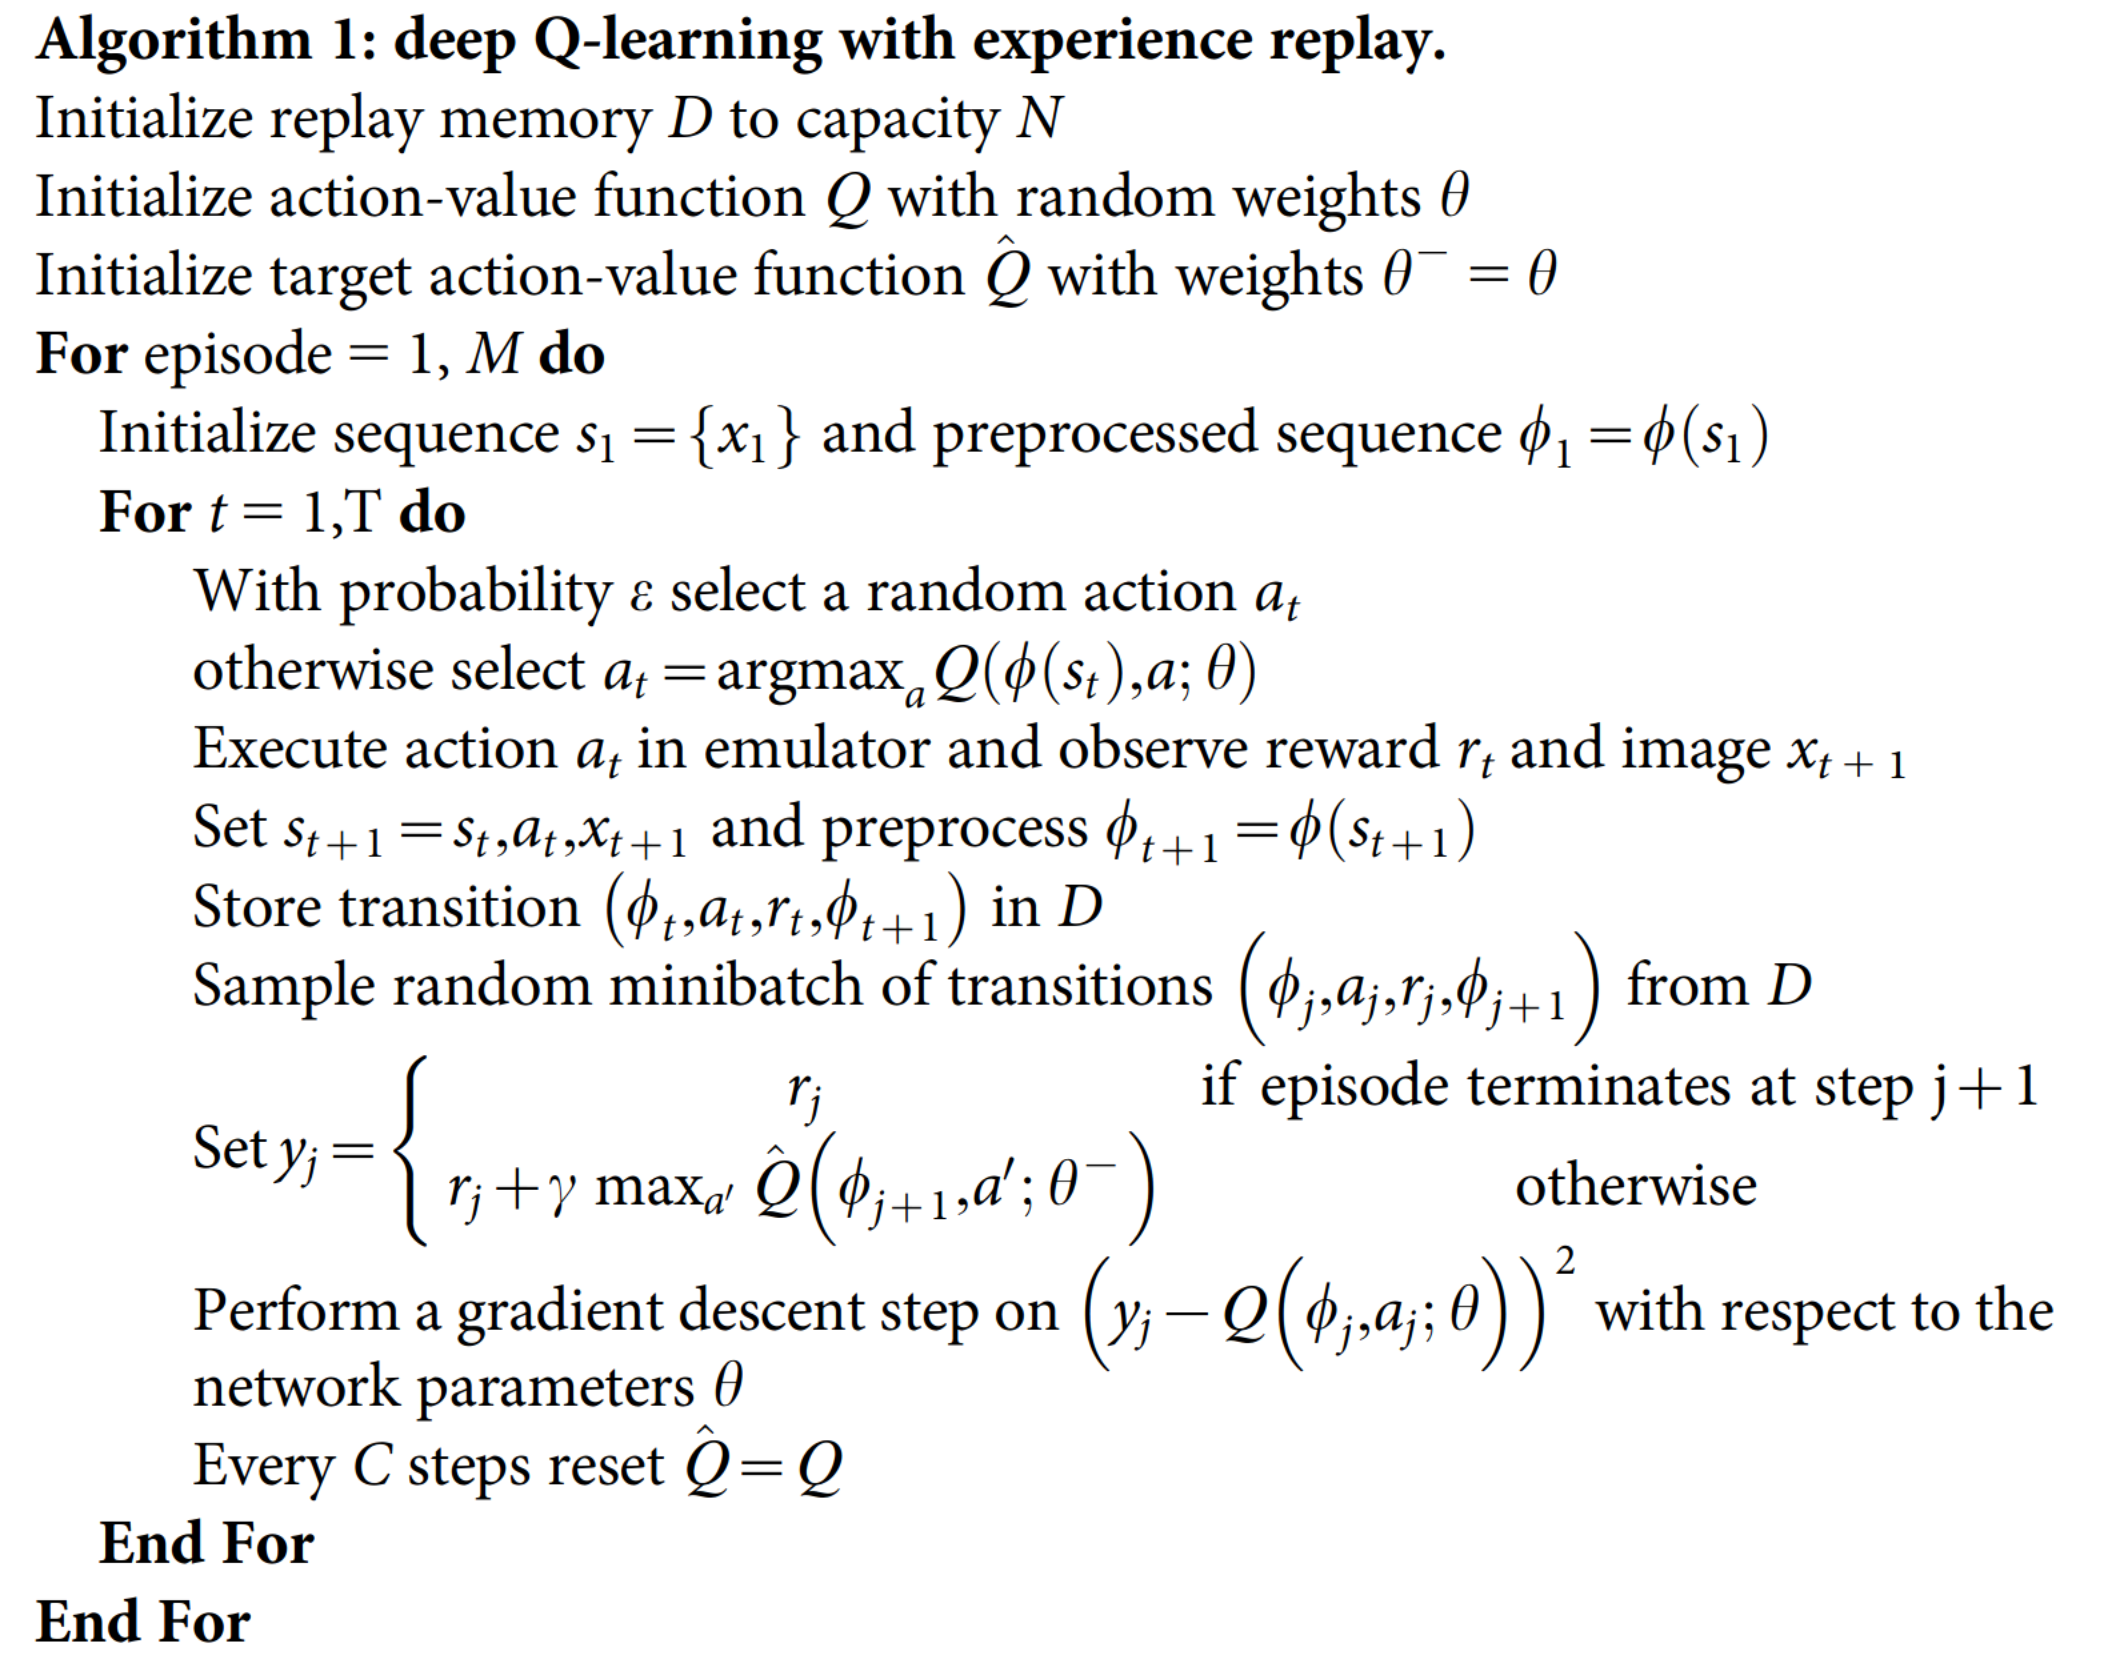
\includegraphics{imgs/dqn_print_1.png}
\caption{DQN paper implementation}
\end{figure}

The Deterministic Policy Gradients, or \texttt{DPG}, is an actor-critic
method that attempts to combine both value-based and policy-based
methods to learn an optimal policy IN continuous action spaces.
Following the original paper,
\href{http://proceedings.mlr.press/v32/silver14.pdf}{Deterministic
Policy Gradient Algorithms}, on the \texttt{DPG}:

\begin{quote}
The deterministic policy gradient has a particularly appealing form: it
is the expected gradient of the action-value function. This simple form
means that the deterministic policy gradient can be estimated much more
efficiently than the usual stochastic policy gradient.
\end{quote}

The \texttt{DDPG} algorithm then is a mix of both \texttt{DPG} and
\texttt{DQN}, where we have two networks: the actor and critic. The
actor is responsible for estimating the value (or action-value) function
while the critic is responsible for evaluating the value function. So
the intuition behind actor-critic methods goes like this:

\begin{enumerate}
\def\labelenumi{\arabic{enumi}.}
\item
  the actor takes in the current state and takes an action, based on the
  current policy \(\pi(a|s;\theta_{\pi})\).
\item
  collect the experience tuple \((s,a,r,s')\) to feed the critic, whose
  job is to estimate \(V(s;\theta_{v})\).
\item
  use the critic output to calculate the advantage function
  \(A(s,a)=r + \gamma V(s';\theta_{v}) - V(s;\theta_{v})\) and use it as
  the new baseline for actor to move on.
\item
  Repeat steps 1 through 3 until a stopping rule is achieved (end
  learning).
\end{enumerate}

But the \texttt{DDPG} algorithm is a bit different from classic
actor-critic methods. The actor in \texttt{DDPG} is used to approximate
\(\max _{a}Q(s_{t+1},a)\), an expression found the original \texttt{DQN}
implementation and not as a learn baseline. So instead of outputting
\(\pi(a|s;\theta_{\pi})\), the actor outputs \(\mu(s;\theta_{\mu})\), an
approximation of \(\max _{a}Q(s_{t+1},a)\) (notice that this is follows
an deterministic policy, not a stochastic policy). Then the critic takes
the actor output and learns to evaluate it, by estimating
\(Q(s,\mu(s;\theta_{\mu});\theta_{Q})\).

Besides that, \texttt{DDPG} is very much like what was described in
steps 1-4. So in the \texttt{DDPG} algorithm implementation of steps 1
through 4 the actor will have two neural networks (a target and a policy
network, like in the \texttt{DQN}) and for the critic we also have two
neural networks (a target and a policy network, also like in the
\texttt{DQN}). Also present in the \texttt{DDPG} algorithm is the replay
buffer, in order improve learning by collecting some chunks of episodes.
Also present are the fixed q targets used to help stabilize learning, as
described in the \texttt{DQN} implementation. \texttt{DDPG} pretty much
resembles the \texttt{DQN} algorithm, but addapted to support continuous
action spaces. The \texttt{DDPG} is depicted in Figure 02.

\begin{figure}
\centering
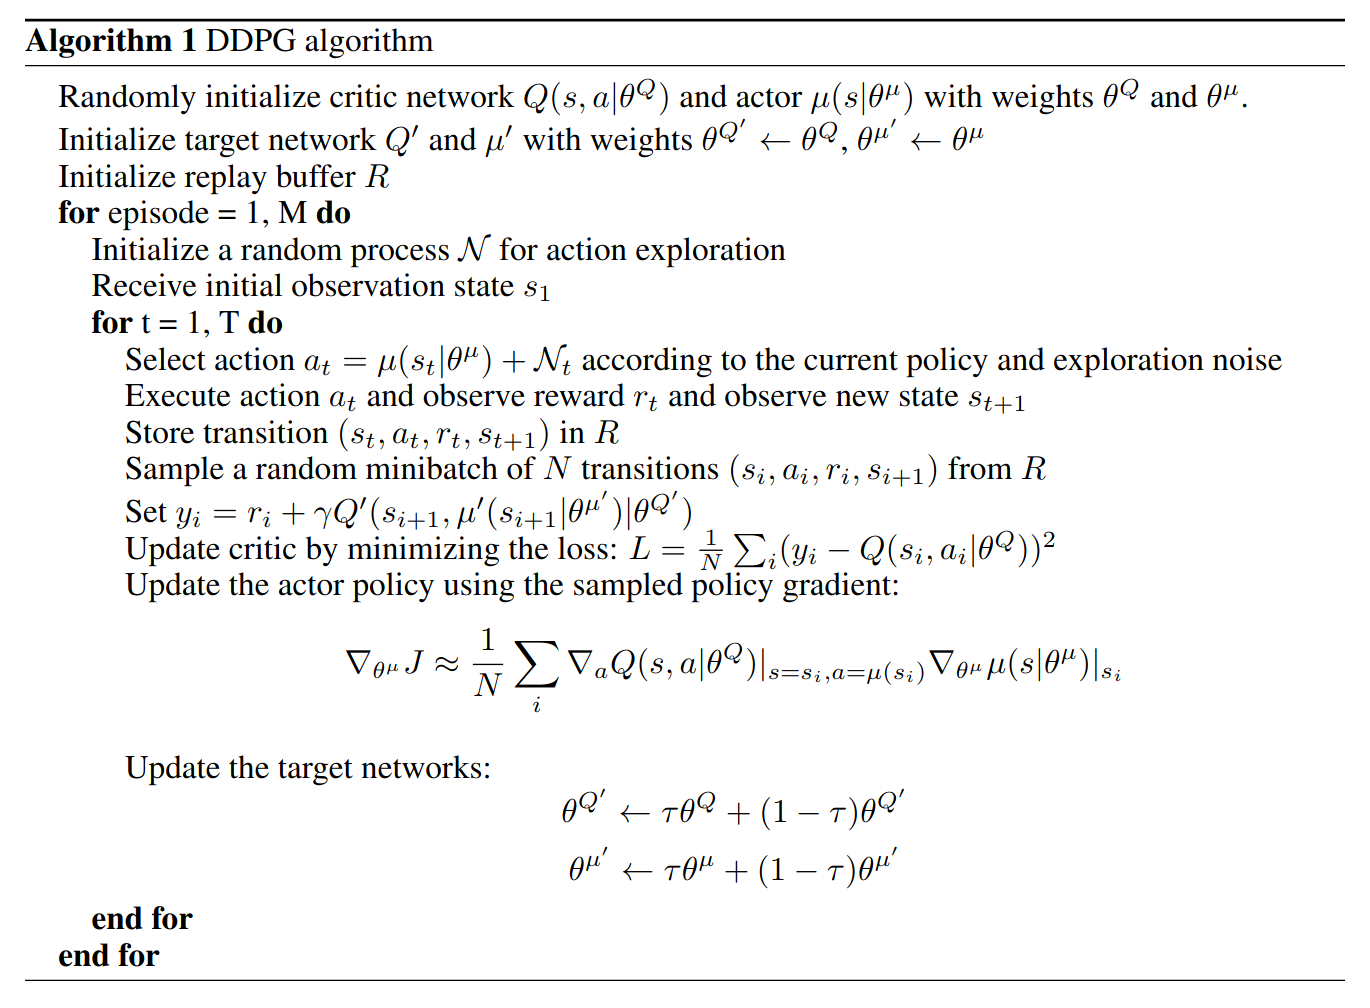
\includegraphics{imgs/ddpg_print_1.png}
\caption{DDPG paper implementation}
\end{figure}

\pagebreak

\hypertarget{coding-the-algorithm-need-to-update}{%
\section{Coding the Algorithm {[}NEED TO
UPDATE{]}}\label{coding-the-algorithm-need-to-update}}

The code implementation of the algorithm used here is mostly inspired
the by ``Pendulum'' project notebook provided by \texttt{Udacity}, in
the ``Policy-Based'' section. Here is a brief description of the files:

\begin{itemize}
\item
  \textbf{Reacher.ipynb}: a jupyter notebook that serves as a wrapper of
  smaller functions. This is the main file, responsible for: 1) starting
  the environment; 2) loading the neural network architecture in
  \texttt{model\_py}; 3) loading the \texttt{dqn\_agent} implementation
  with fixed q-targets and experience replay.
\item
  \textbf{model.py}: this is where the neural network architecture is
  stored, written in \texttt{pytorch}.
\item
  \textbf{dqn\_agent.py}: this is code that implements the \texttt{DQN}
  high-level ideas of fixed q-targets and experience replay.
\item
  \textbf{checkpoint.pth}: this is the \texttt{DQN} model weights used
  to solve the environment \textbf{with} early stopping (which means
  that if achieve the average score of +13 over 100 episodes than we
  finish learning).
\item
  \textbf{checkpoint\_no\_callback.pth}: this is the \texttt{DQN} model
  weights used to solve the environment \textbf{without} early stopping
  (which means that even if achieve the average score of +13 over 100
  episodes, we still continue learning until we hit the total number of
  episodes specified).
\end{itemize}

\hypertarget{comments-on-model.py}{%
\subsection{\texorpdfstring{Comments on
\texttt{model.py}}{Comments on model.py}}\label{comments-on-model.py}}

The \texttt{model.py} file contains the \texttt{pytorch} model
architecture used to solve the environment. The architecture used is a
simple 2 fully connected layer with RELU activation function. The input
size that the network expects is the 37 dimension array corresponding to
the state space size, while the output layer is a simple linear layer
with output size of 4 which corresponds to the 4 actions available
(forward,backward,left,right).

The \texttt{hyperparameters} used are:

\begin{itemize}
\tightlist
\item
  the number of units in both first and second fully connected layer are
  64.
\item
  the learning rate parameter used in the \texttt{adam} optimizer is
  \texttt{LR\ =\ 5e-4} (this actually belongs to the \texttt{model.py}
  file, but it's also part of the neural network architecture)
\end{itemize}

\hypertarget{comments-on-dqn_agent.py}{%
\subsection{\texorpdfstring{Comments on
\texttt{dqn\_agent.py}}{Comments on dqn\_agent.py}}\label{comments-on-dqn_agent.py}}

The \texttt{model.py} file contains:

\begin{itemize}
\tightlist
\item
  the \texttt{hyperparameters} used:

  \begin{itemize}
  \tightlist
  \item
    \texttt{BATCH\_SIZE\ =\ 64}: neural network mini-batch size
  \item
    \texttt{GAMMA\ =\ 0.99}: the discount factor used in the discounted
    sum of rewards
  \item
    \texttt{TAU\ =\ 1e-3}: the \(\tau\) parameter used to soft update of
    target parameters
  \item
    \texttt{LR\ =\ 5e-4}: the neural network learning rate use in
    gradient descent
  \item
    \texttt{UPDATE\_EVERY\ =\ 4}: how often to update the network
  \item
    \texttt{BUFFER\_SIZE\ =\ 1e5}: replay buffer size (how much we store
    into the replay buffer)
  \end{itemize}
\item
  the \texttt{Agent} class:

  \begin{itemize}
  \tightlist
  \item
    implements the \texttt{step}, \texttt{act}, \texttt{learn} and
    \texttt{soft\_updates} methods
  \item
    initializes the policy and target networks for fixed q-target
    strategy
  \item
    initializes the \texttt{ReplayBuffer} class.
  \end{itemize}
\item
  the \texttt{ReplayBuffer} class: an API to

  \begin{itemize}
  \tightlist
  \item
    initialize storage
  \item
    implement the \texttt{add} (add new experiences) and \texttt{sample}
    (sample experiences to mini-batch GD learning) methods
  \end{itemize}
\end{itemize}

\pagebreak

\hypertarget{results}{%
\section{Results}\label{results}}

The \texttt{DQN} implementation was able to successfully solve the task
of achieving an average score of +13 over 100 episodes in 445 episodes.
Its average score was 13.01, as shown in the \texttt{Figure\ 02} bellow.
It's important to note that we used a early stopping technique not to go
into the 5000 episodes, if not needed. The plot of the scores is shown
in \texttt{Figure\ 03} and it suggests that just increasing the number
of episodes alone could improve performance.

After seeing the plot shown in \texttt{Figure\ 03} I've tried to improve
the agent's performance by just removing the early stopping if-clause
and letting the DQN to train the entire 3000 episodes. The results are
shown in the \texttt{Figure\ 04} and from it we can see that increasing
the number of episodes can only get us so far (because the average score
stagnates after about 1000 episodes) and to make the agent learn better
we have to try different strategies, as suggest in the section Ideas to
Explore Later.

\pagebreak

\hypertarget{ideas-to-explore-later}{%
\section{Ideas to Explore Later}\label{ideas-to-explore-later}}

Some ideas that could lead to improvements in the learning process are
trying to:

\begin{itemize}
\item
  Use Double Q-Learning, as presented
  \href{https://arxiv.org/pdf/1509.06461}{here}. The idea is very
  similar the the DQN, but the Q-learning algorithm is known to
  overestimate action values under certain conditions and so double
  Q-learning could lead to better performance.
\item
  Change the neural network architecture. Maybe add a convolutional
  layer or some dropout and see how things go.
\item
  Try using \href{https://arxiv.org/pdf/1511.05952}{prioritized
  experience replay} to replay important transitions more frequently,
  and therefore learn more efficiently.
\item
  Try Dueling DQN, as presented
  \href{https://arxiv.org/pdf/1511.06581}{here}. The idea is to
  introduce the advantage function as a separate estimator. The main
  benefit it provides is to generalize learning across actions without
  imposing any change to the underlying reinforcement learning
  algorithm. The results displayed in the paper shows that this
  architecture could lead to better policy evaluation in the presence of
  many similar-valued actions
\end{itemize}

\end{document}
